\documentclass[11pt,a4paper]{article}
\usepackage[utf8]{inputenc}
\usepackage{graphicx,enumitem}

\title{Ray Tracer application Initial Report}
\author{A. Manolache, N. Shirvanian, A. Georgiou, S. Orazgulyyev, S. Moraby}
\date{February 5, 2018}
\begin{document}
\maketitle

\section{Introduction}

This report will aim to provide a succinct, but comprehensive, description of our ray tracer implementation strategy for the Group Project module, an outline of the goal currently achieved, and obstacles that were met. The general idea behind the decision for our project's architectural design will be defined so that the motivation is well understood, as well as our future milestones. Finally, an analysis of our team's organization will be provided followed by a discussion in the conclusion.

\section{Project Description}

The aim of our project is to construct a well-defined ray tracer application that will go beyond a simple implementation. The following sections aim to provide further information on the design of our system and the milestones set to achieve the production of the final software. 

\subsection{Project Design}

The decision as a group was to approach the project's design from a Model-View-Controller (MVC) architecture angle. This will enable us to have our software constructed from interconnected, but separated components, which in turn will allow for greater flexibility in our development life cycle. In our current situation we identified two major software components that serve as the main building block of our final project:

\begin{itemize}[nosep, wide=20pt, leftmargin=*, after=\strut]
    \item The GUI, which will be responsible for allowing the user to interact with the drawing canva
    \item The backend server which will feed the data received from the GUI to our ray tracer and process it
\end{itemize}

Taking into account the group's programming aptitudes and technical knowledge, we decided to build the GUI using JQuery and HTML5 while the back-end of the web application will be implemented using Java 8 with additional integration frameworks as well as a Tomcat server. In anticipation of our project growing in scalability we planned to integrate a Spring framework in order to help us keep the structure of our project as decoupled and modular as possible. Spring components such as the Spring MVC can assist us in separating the building blocks of our application and the integration of the Rest Full services. In addition, its inversion of control container can deal, via dependency injection, with the life cycle management of our Java objects.

In a nutshell, our program's workflow can be described as follows:
\begin{itemize}[nosep, wide=20pt, leftmargin=*, after=\strut]
    \item Firstly an Ajax call will trigger the sending of the image from the GUI component in a JSON format
    \item This will then map the JSON payload to a Plain Old Java Object (POJO) and feed it to our ray tracing algorithm
\end{itemize}

\subsection{Milestones}

The development life cycle of our project will revolve around achieving the milestones as shown in the chart below:
\begin{enumerate}[nosep, wide=20pt, leftmargin=*, after=\strut]
    \item Build the GUI prototype 
    \item Build the back end server
    \item Allow the GUI to send JSON payloads to the server
    \item Build a Basic Ray-tracing Algorithm and feed it data from the GUI
    \item Improve the GUI by allowing the use of multiple shapes and other functionalities
    \item Integrate advanced rendering techniques such as, but not limited to, anti-aliasing, depth of field, specular and diffuse shading
\end{enumerate}


\begin{figure}[h]
\centering
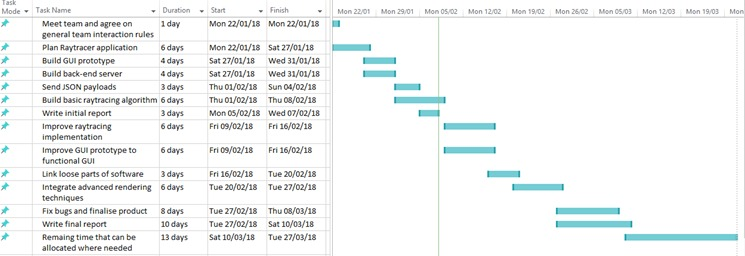
\includegraphics[scale = 0.4]{ganttchart.jpeg}
\caption{Grantt Chart}
\end{figure}

\subsection{Progress}

In essence, a functional ray tracer application has been set up so far as the first three objectives have been accomplished. Over and above that the GUI prototype has been linked to the back end server where it sends JSON payloads to the server. We are currently working on building a basic ray-tracing algorithm and then we will proceed to make further improvements to our application. 

\section{Project Organization}

This section explores how we are going to be dealing with the evolving dynamics of working as a team; five different personalities and minds, coming together to achieve an ultimate goal in the most efficient way feasible. Our adopted methodology is defined as being agile since our ideas and implementation strategies are expected to change under the collaborative effort of our team. Keeping in mind this expectation, our team is ready to face future changes, challenges and issues that may surface and overcome these as fast as possible. 

\subsection{Group Interactions and roles}

Together we create a team of five individuals, each with their own different skills and level of expertise on the number of languages that will be used throughout the project’s lifecycle. Each member will be undertaking a part in the production of the software, taking into account the member’s level of pre-existing knowledge in creating such part. We have decided to allow four members to work on the back end for the beginning of the project, since the back end forms the most important part for the correct operation of the final product. Nima will be working on creating the code for the GUI that will later be connected to the back end with Andrei’s help. Additionally, Antria, Andrei, Suleyman and Suhaila will be mainly working on the ray tracing algorithm and its successful implementation. All team members have agreed to approach and tackle the problem in an agile manner, allowing us to jump where and when needed to help other team members, while still working on our assigned positions, throughout the development of the software. Additionally, we trust all team members to manage their time effectively and to inform the team in time, if they believe that their schedule will potentially become overwhelming and will lead to delays of the completion of their task.

Furthermore, we will keep assigning regular meetings with the team, every week, to discuss issues that have come up, ask for help and keep up to date on the general progress of the project and the milestones set. We will be gradually completing the aims set in the Project Description, tackling each one in a timely manner and at the pace that everyone is comfortable in. In the unfortunate case that the work assigned to a member is not completed in time, we will assign additional members on that specific task and re-evaluate the deadline of that task. All progress and changes of the source code will be uploaded on GitHub, where all team members will be able to view, review and comment on the work. Moreover, a private group chat is being used to discuss any further questions and ideas, provide useful links to tutorials, set up meetings and generally keep up to date every day until our next meeting.

\subsection{Peer Assessment and Conflict Resolution}

Peer assessment for this project, will be conducted not based on the final result, but based on the overall work and contribution, of each member of our team, throughout the time dedicated to the completion of the final product. However, we do not expect to assess the work done, by other group members, based on the quality or amount of the source code that they have produced. It is our understanding that each member possesses different sets of skills; therefore it is also our goal not to only complete this challenging project, but to also learn and become better from it. Moreover, the peer assessment will be conducted taking into account the willingness of members to help out in any possible way and their availability and respondence throughout the next few weeks until the deadline. Dealing with the completion of tasks, good time management, continuous communication and ability to work with others effectively are also substantial considerations that will influence the peer assessment.

Nevertheless, healthy competition is always welcome as long as it is nothing but healthy. Our team expects that differences in opinions will surface but has also agreed that unfriendly behaviour will not be tolerated. In the event of a conflict, we have decided to keep in mind that:

\begin{itemize}[nosep, wide=20pt, leftmargin=*, after=\strut]
    \item we all have the same goal 
    \item we only use reason before raising an argument
    \item we are all entitled to our own opinion and only express it kindly
    \item we care about our team members’ feelings 
    \item we all have to compromise sometimes 
    \item we are not always right
\end{itemize}

Always considering the above, we are confident that even if conflicts do arise, we will be able to resolve them with success.

\section{Conclusion}

Ultimately the expected outcome of this report is a sophisticated and intriguing implementation of a ray tracer that will comprise of a number of different techniques, each one playing an essential role in the successful operation of the product. Additionally, it is our goal to create a GUI that allows options (change of colour, shape) to the user and an improved ray-tracing algorithm that is not limited to the use of just one shape. Moreover, our goal as a team is to come together, learn and overcome any obstacles that come with developing software. Finally, we are all prepared and eager to experience and adapt to the general challenges of the industry.

\end{document}
